\documentclass[aspectratio=169]{ctexbeamer}
\usepackage[T1]{fontenc}
\usepackage{latexsym,amsmath,xcolor,multicol,booktabs,calligra}
\usepackage{graphicx,listings,stackengine}
\usepackage{hyperref}

\usepackage{PekingU}

% 去掉每节/子节前面的自动目录页
\AtBeginSection[]{}
\AtBeginSubsection[]{}

% ===== 每节课改这里 =====
\author{Cap1taL}
\title{数据结构 1}
\subtitle{中国人能飞，不是不飞，是缓飞，慢飞，优飞；不是不让谁飞，是让有能力的人先飞，让先飞的人带后飞——这才是有次序的飞，有温度的飞}
\date{2026年8月}
% ========================

% 代码高亮设置
\definecolor{deepblue}{rgb}{0,0,0.5}
\definecolor{deepred}{rgb}{0.6,0,0}
\definecolor{deepgreen}{rgb}{0,0.5,0}
\definecolor{halfgray}{gray}{0.55}

\lstset{
    basicstyle=\ttfamily\small,
    keywordstyle=\bfseries\color{deepblue},
    emphstyle=\ttfamily\color{deepred},
    stringstyle=\color{deepgreen},
    numbers=left,
    numberstyle=\small\color{halfgray},
    rulesepcolor=\color{red!20!green!20!blue!20},
    frame=shadowbox,
}

\begin{document}

\kaishu

% 封面
\begin{frame}
    \titlepage
\end{frame}

% 目录
% \begin{frame}{目录}
%     \tableofcontents[sectionstyle=show,subsectionstyle=show/shaded/hide,subsubsectionstyle=show/shaded/hide]
% \end{frame}

% ===== 从这里开始写你的内容 =====

\section{线段树}

\subsection{常用算法}
\begin{frame}{线段树动态开点}
    \begin{itemize}
        \item 用于维护的范围较大，不能完整建树的情况
        \item 基本思想是修改时涉及到的点才分配内存
        \item 一般使用数组实现，指针会比较缓慢
        \item 具体实现可以善用引用来简化代码
        \item Code：\url{https://www.luogu.com.cn/record/291318185}
        \item 动态开点是一种很重要的技术，后面还会用到
    \end{itemize}
\end{frame}
\begin{frame}{线段树合并}
    \begin{itemize}
        \item 即我们需要得到一颗新的树，其各个节点都为原来两棵树的信息合并结果
        \item 我们显然不能每次都建满一颗树，因此线段树合并需要使用动态开点
        \item 线段树合并实际上相当暴力：同时在两棵树上 DFS，若某个儿子只有某个树有，则直接 “指向” 那个儿子而不向它递归
        \item 考虑这样操作的复杂度，每次合并最多经过较小树的点数，且合并完后可认为我们遍历过的位置都 “删除” 了
        \item 因此总时间复杂度是总点数量级，一般为 $O(n\log V)$
        \item 可以垃圾回收
        \item Code：\url{https://www.luogu.com.cn/record/106948561}
    \end{itemize}
\end{frame}

\begin{frame}{线段树分裂}
    \begin{itemize}
        \item 即我们需要得到一颗新的树，其包括原树 $[l,r]$ 内所有的信息，且原树上的这部分信息删除
        \item 在树上找到我们需要的区间，建立上方所有的相关点，断开原树上的连边，让新节点指向当前节点即可
        \item 代码形如区间修改，复杂度 $O(\log n)$
        \item Code：\url{https://www.luogu.com.cn/record/106948561}
    \end{itemize}
\end{frame}

\begin{frame}{李超线段树}
    % 整行居中布局
    \centering
    % 左侧图片区域 占 0.48 文本宽
    \begin{minipage}{0.48\textwidth}
    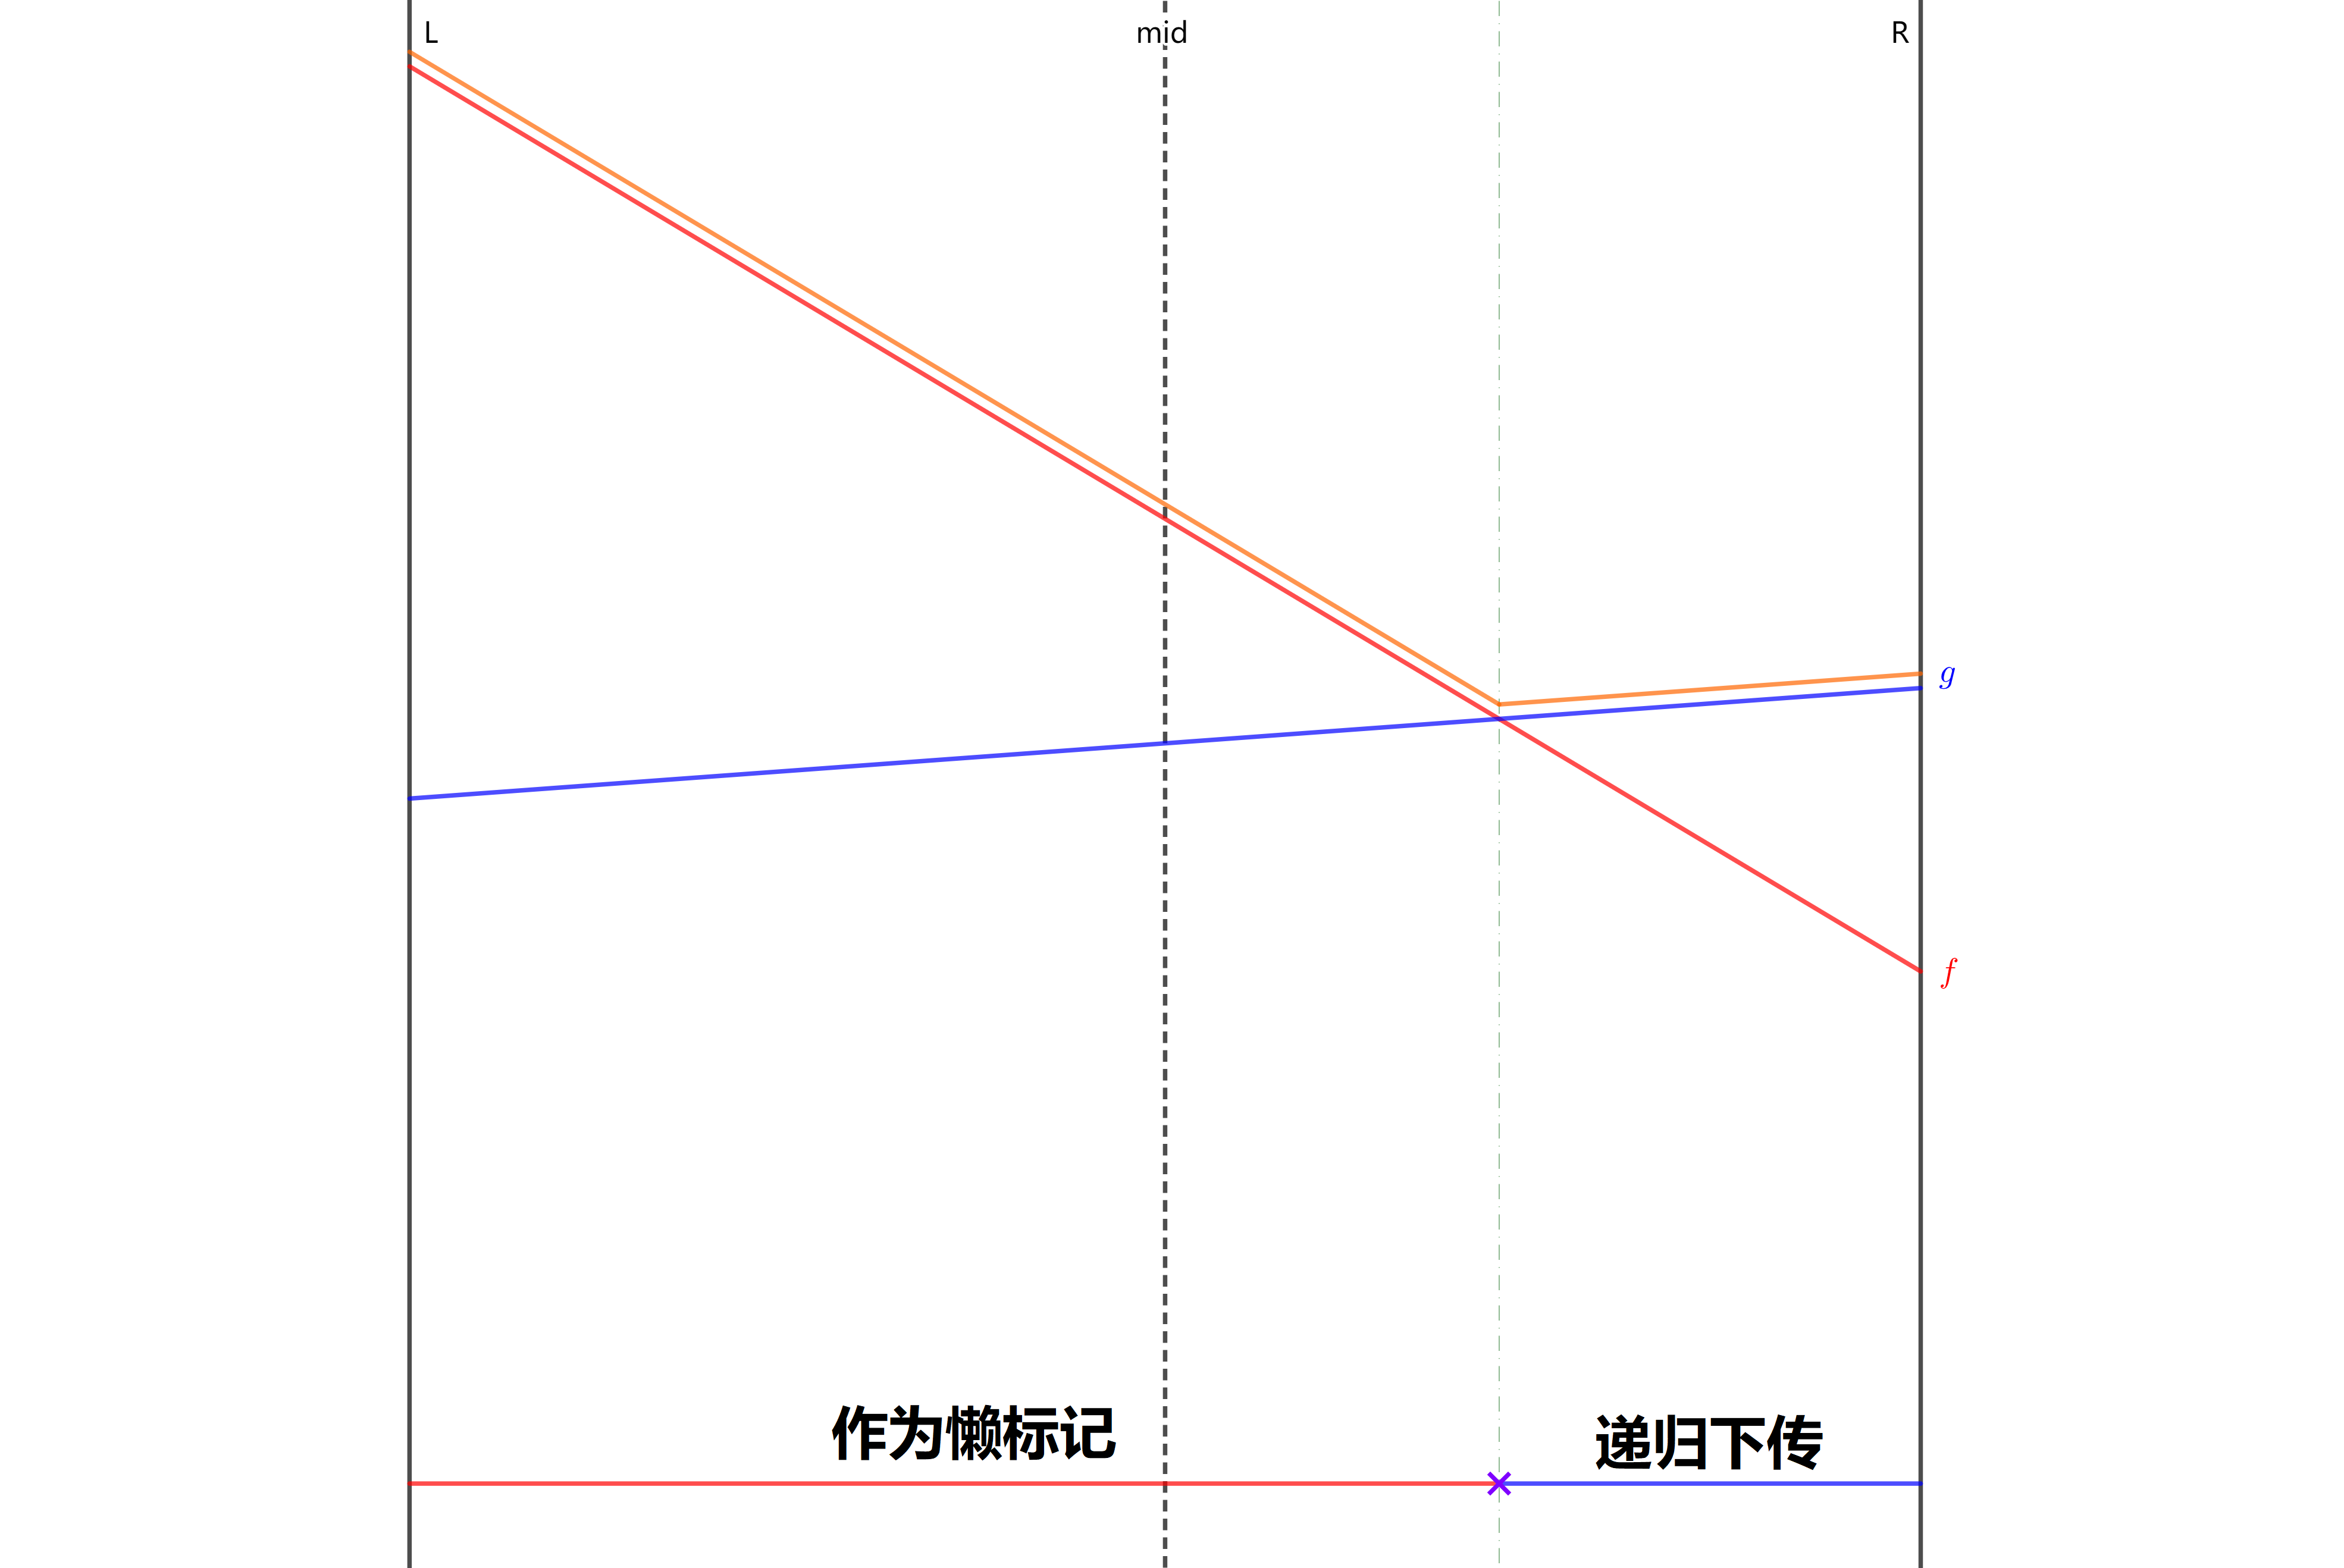
\includegraphics[width=\linewidth]{pic/li-chao-tree-1.png}
    \end{minipage}
    \hfill % 中间留白分隔
    % 右侧文字区域
    \begin{minipage}{0.50\textwidth}
        \begin{itemize}
            \item 一页讲懂李超线段树
            \item 标记永久化，每个节点上维护一个线段 $x$（定义域完全包含当前节点）
            \item 当上方传入一条线段 $y$ 时
            \begin{itemize}
                \item 若区间内 $y$ 完全在 $x$ 下面，则它没用，直接丢弃
                \item 若区间内 $y$ 完全在 $x$ 上面，则它很牛，直接舍弃 $x$ 让 $y$ 上位
                \item 若它们存在交点，则把中点处牛的留下，另一个继续向交点区间递归
            \end{itemize}
        \end{itemize}
    \end{minipage}
\end{frame}

\begin{frame}{李超线段树}
    % 整行居中布局
    \centering
    % 左侧图片区域 占 0.48 文本宽
    \begin{minipage}{0.48\textwidth}
    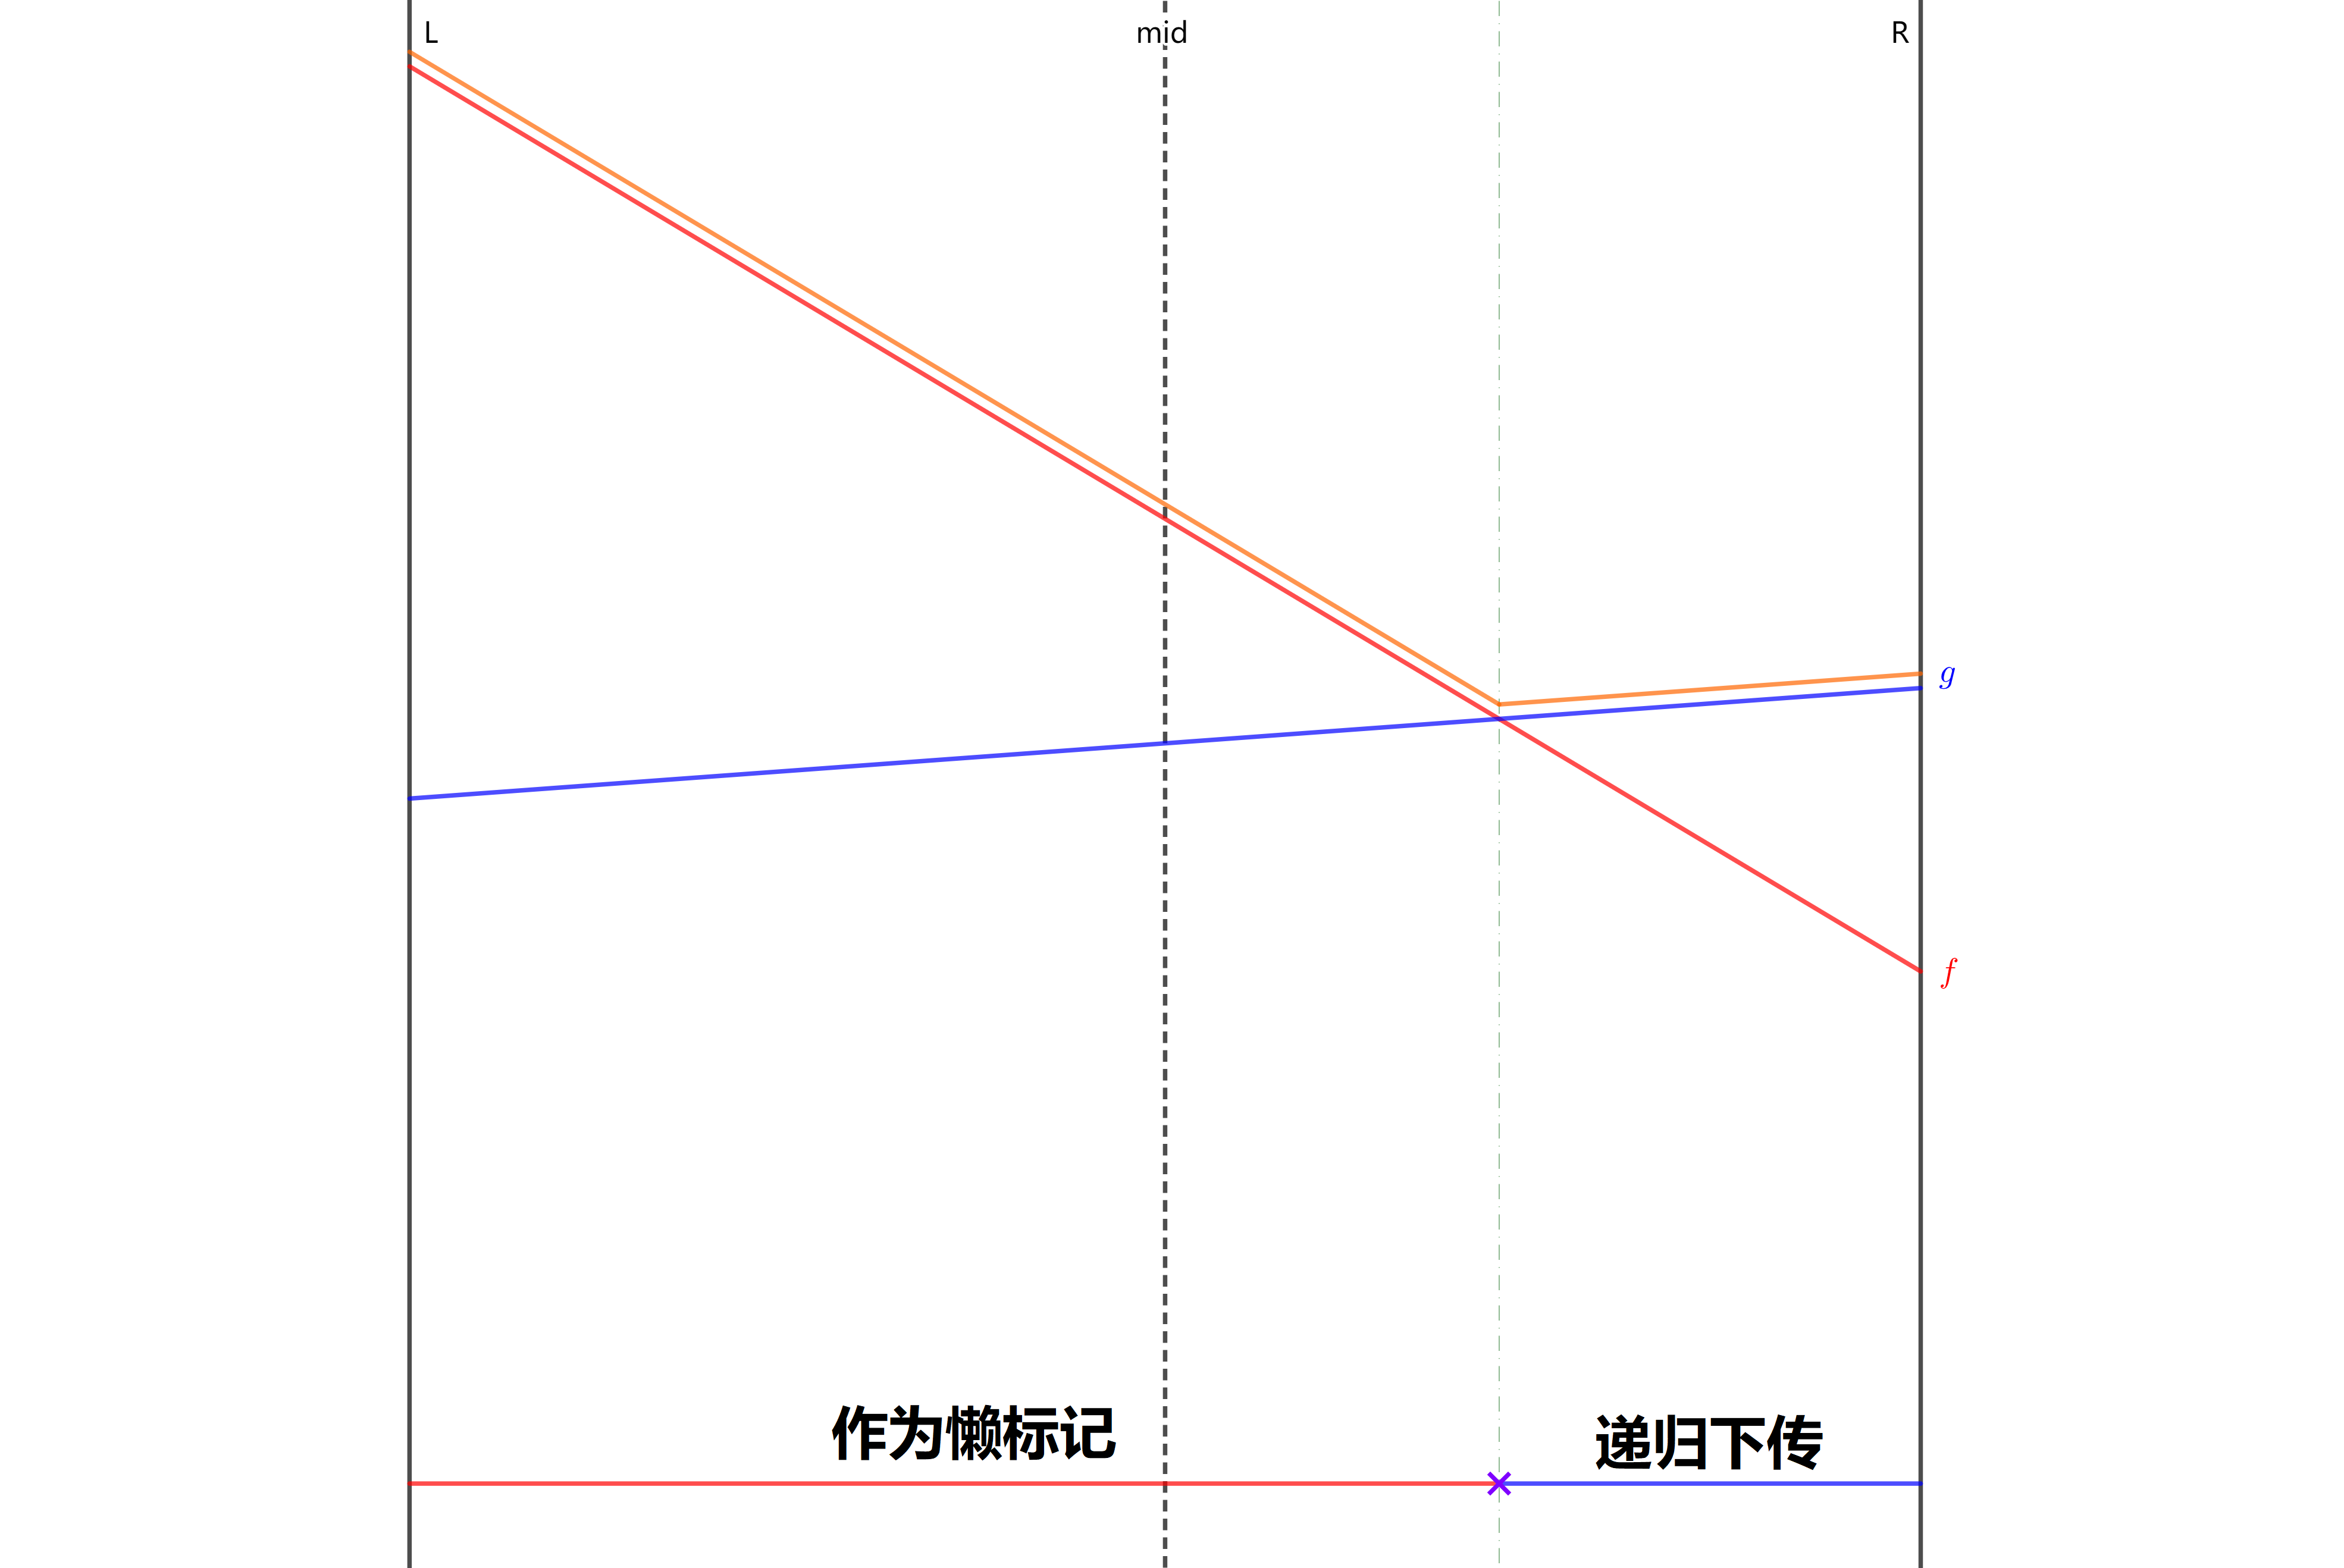
\includegraphics[width=\linewidth]{pic/li-chao-tree-1.png}
    \end{minipage}
    \hfill % 中间留白分隔
    % 右侧文字区域
    \begin{minipage}{0.50\textwidth}
        \begin{itemize}
            \item 若插入直线，则复杂度显然为 $O(\log n)$
            \item 若插入线段，则我们需要先定位到 $O(\log n)$ 个区间，再执行插入直线的操作。复杂度 $O(\log^2 n)$
            \item 查询显然是 $O(\log n)$ 的
            \item 若对其使用线段树合并，问题在于需要在重叠部分下传线段。注意到我们只会向下移动线段或者将其删除，因此复杂度是有保证的
        \end{itemize}
    \end{minipage}
\end{frame}

\begin{frame}{可持久化线段树}
    \begin{itemize}
        \item 所谓可持久化，即是我们每次修改后都会建立一个新版本，要求支持在任意版本上查询信息
        \item 朴素做法是每次都把数据结构完整拷贝一次
        \item 对于线段树，我们有更好的做法。注意到一次修改涉及到的点是有限的，我们可以只新建立这些相关节点，同时 “复用” 未修改的节点，直接让新节点的儿子指针指向它们即可
        \item 可以发现，在可持久化线段树中，一个节点可能会被多个版本使用。我们正是通过这种手段来降低复杂度的
        \item 具体实现与动态开点类似。
        \item Code：\url{https://www.luogu.com.cn/record/291331658}
    \end{itemize}
\end{frame}

\begin{frame}{可持久化线段树}
    \begin{itemize}
        \item 上面所提到的修改均为单点修改
        \item 对于区间修改，一般的懒标记便会失效，原因是显然的：懒标记下传会破坏节点的共享结构
        \item 因此，若需要支持区间修改，必须进行标记永久化
        \item 标记永久化不再存在 push\_down 函数，而是在修改时直接维护途径所有的值，并在最下方打上标记，用于将修改告知子树内的点
        \item 查询时，需要考虑节点上方所有的标记——他们是没有被下传、被永久化在上方的，因此需要补上它们的贡献
    \end{itemize}
\end{frame}

\begin{frame}{线段树单侧递归}
    \begin{itemize}
        \item 有时我们难以直接合并两侧的答案
        \item 此时我们可以尝试不要求 push\_up 是 $O(1)$
        \item 如果可以在 $O(\log n)$ 的时间内进行 push\_up，也可以在 $O(\log^2n)$ 的时间内完成维护
    \end{itemize}
\end{frame}


\section{平衡树}
\subsection{简单平衡树操作}
\begin{frame}{使用 \texttt{\_\_gnu\_pbds::tree} 维护简单的平衡树操作}
    \begin{itemize}
        \item 可以当做加强版的 \texttt{set}。
        \item 需要包含头文件 \texttt{<bits/extc++.h>}
        \item 先引入命名空间：\texttt{using namespace \_\_gnu\_pbds;}
        \item 原生支持扩展接口：\texttt{order\_of\_key()}、\texttt{find\_by\_order()}；
              \textbf{注意：该红黑树容器不自带 \texttt{split}、\texttt{join} 操作}
        \item 示例代码：\url{https://www.luogu.com.cn/record/291148652}
    \end{itemize}
\end{frame}

\subsection{自定义平衡树节点更新器}
\begin{frame}{自定义 \texttt{\_\_gnu\_pbds::tree} 的更新策略来维护序列问题}
    \begin{itemize}
        \item 自定义 Node_update，可以在平衡树上维护自己需要的信息，也可以自己访问平衡树上的所有点进行查询
        \item 这使得可以不关注平衡树的平衡部分，只把它当做一颗自动平衡的二叉搜索树来使用。
        \item pbds 内置了红黑树，跑起来相当快，甚至也同步支持键值映射
        \item 详情见习题
    \end{itemize}
\end{frame}


\section{树套树}

\begin{frame}{树套树}
    \begin{itemize}
        \item 在外层树的每个节点上维护一个内层树
        \item 外层树常使用线段树或树状数组
        \item 内层树常为 STL 容器（平衡树），若内层使也用线段树，一般必须使用动态开点
        \item 树套树可以在线处理一类二维操作，它可以把一个矩形拆为 $O(\log^2 n)$ 块
    \end{itemize}
\end{frame}
















\section{习题}

\subsection{洛谷 P3834 【模板】静态区间第 k 小}

\begin{frame}{洛谷 P3834 【模板】静态区间第 k 小}
    给定一个长度为 $n$ 的整数序列 $a$，有 $m$ 次查询，每次查询闭区间 $[l,r]$ 内的第 $k$ 小值。
    
    $1\le n,m\le 2\times10^5$，$0\le a_i\le 10^9$
\end{frame}

\begin{frame}{Solution}
    \begin{itemize}
        \item 在值域上考虑
        \item 按照序列下标依次插入元素到值域数据结构，同时可持久化
        \item 现在我们已经可以利用前缀可持久化，支持所有 $l=1$ 的前缀询问，只需要维护范围内数的个数，再在对应版本上线段树二分即可
        \item 对于区间询问，考虑类似差分地处理
        \item 同时在两棵树上线段树二分，访问的 “数的数量” 永远用两个版本相减得到
        \item 复杂度 $O(n\log n)$
    \end{itemize}
\end{frame}

\subsection{洛谷 P3402 【模板】可持久化并查集}

\begin{frame}{洛谷 P3402 【模板】可持久化并查集}
    $n$ 个集合初始时第 $i$ 个集合仅含数 $i$。共 $m$ 次操作，支持：
    \begin{itemize}
        \item \texttt{1 a b}：合并 $a,b$ 所在集合；
        \item \texttt{2 k}：回到第 $k$ 次操作之后的状态（$k=0$ 回到初始状态）；
        \item \texttt{3 a b}：询问 $a,b$ 是否属于同一集合，是则输出 $1$，否则输出 $0$。
    \end{itemize}

    $1\le n\le 10^5$，$1\le m\le 2\times 10^5$，$1\le a,b\le n$。
\end{frame}

\begin{frame}{Solution}
    \begin{itemize}
        \item 思考可持久化线段树可以支持什么操作——实质上就是可持久化数组
        \item 使用可持久化线段树暴力可持久化一切操作即可
        \item 需要注意不能使用路径压缩，因为它的复杂度是基于均摊的
        \item 使用复杂度稳定为 $O(\log n)$ 的按秩合并即可
    \end{itemize}
\end{frame}

\subsection{洛谷 P3380 【模板】树套树}

\begin{frame}{洛谷 P3380 【模板】树套树}
    维护长度为 $n$ 的数列，支持 $m$ 次操作：
    \begin{itemize}
        \item \texttt{1 l r k}：查询 $k$ 在区间 $[l,r]$ 内的排名；
        \item \texttt{2 l r k}：查询区间 $[l,r]$ 内排名为 $k$ 的值；
        \item \texttt{3 pos k}：将 $pos$ 位置的数修改为 $k$；
        \item \texttt{4 l r k}：查询区间 $[l,r]$ 内 $k$ 的前驱（严格小于 $k$ 的最大值，不存在输出 $-2147483647$）；
        \item \texttt{5 l r k}：查询区间 $[l,r]$ 内 $k$ 的后继（严格大于 $k$ 的最小值，不存在输出 $2147483647$）。
    \end{itemize}
    
    $1\le n,m\le 2\times 10^5$，值域 $[0,10^8]$。
\end{frame}

\begin{frame}{Solution}
    \begin{itemize}
        \item 线段树套平衡树
        \item 在线段树每个节点维护一个平衡树，内部管理当前区间的所有数字
        \item 一个数字只会存在于 $O(\log n)$ 个平衡树中，借此可以分析大部分操作的复杂度为 $O(\log^2 n)$
        \item 特别注意操作二，我们需要先二分一个值，然后转化为操作一，因此复杂度为 $O(\log^3 n)$
    \end{itemize}
\end{frame}

\subsection{【模板】动态区间第 k 小}

\begin{frame}{【模板】动态区间第 k 小}
    给定长度为 $n$ 的序列，支持 $m$ 次操作：
    \begin{itemize}
        \item \texttt{Q l r k}：查询下标在 $[l,r]$ 中第 $k$ 小的数；
        \item \texttt{C x y}：将 $a_x$ 修改为 $y$。
    \end{itemize}
    
    $1\le n,m\le 10^5$，$1\le l\le r\le n$，$1\le k\le r-l+1$，$1\le x\le n$，$0\le a_i,y\le 10^9$。
\end{frame}

\begin{frame}{Solution}
    \begin{itemize}
        \item 即只有【模板】树套树 的操作 2,3
        \item 采用线段树套线段树可以做到 $O(\log^2n)$，优于线段树套平衡树的 $O(\log^n)$
        \item 具体地，我们可以同时处理 $O(\log n)$ 棵内层线段树，同时在所有树上进行线段树二分
        \item 为了减小常数，可以在外层使用树状数组，并没有本质改变
    \end{itemize}
\end{frame}

\subsection{洛谷 P4198 楼房重建}

\begin{frame}{洛谷 P4198 楼房重建}
    小 A 在 $(0,0)$ 处观察。第 $i$ 栋楼房为连接 $(i,0)$ 和 $(i,H_i)$ 的线段，其中 $H_i$ 为其高度。

    若某栋楼房上存在一个高度大于 $0$ 的点，使得它与 $(0,0)$ 的连线没有与之前的楼房相交，则这栋楼房可见。

    初始时所有楼房高度均为 $0$。共有 $M$ 次操作，每次将横坐标为 $X_i$ 的楼房高度改为 $Y_i$。求每次操作后小 A 能看到的楼房数量。

    $1 \le N,M \le 10^5$，$1 \le X_i \le N$，$1 \le Y_i \le 10^9$
\end{frame}

\begin{frame}{Solution}
    \begin{itemize}
        \item 求出每个位置的正切值
        \item 问题转化为：单点修改，查询全局前缀最大值个数
        \item 考虑如何 push\_up。左区间的前缀最大值全部保留，问题在于右侧可能不会保留
        \item 因此我们需要支持 “求一个节点区间内大于 $x$ 的前缀最大值数”
        \item 如何计算？若左区间最大值小于 $x$，则左侧必无贡献，递归到右侧。若左区间最大值不小于 $x$，则右侧所有前缀最大值都必定有效，递归到左侧即可。
        \item Code：\url{https://www.luogu.com.cn/record/291350206}
    \end{itemize}
\end{frame}

% ===== 结束页 =====

\begin{frame}
    \begin{center}
        {\Huge\calligra Thanks!}
    \end{center}
\end{frame}

\end{document}
